\begin{frame}{Exploring How the Three Parameters Change the Response}
\small
The fits did not reproduce the measured frequency and amplitude together.
To better understand their influence, we explored \(C\), \(C_{th}\) and \(S_e\) across a parameter grid.
\par\vspace{0.10cm}
\centering
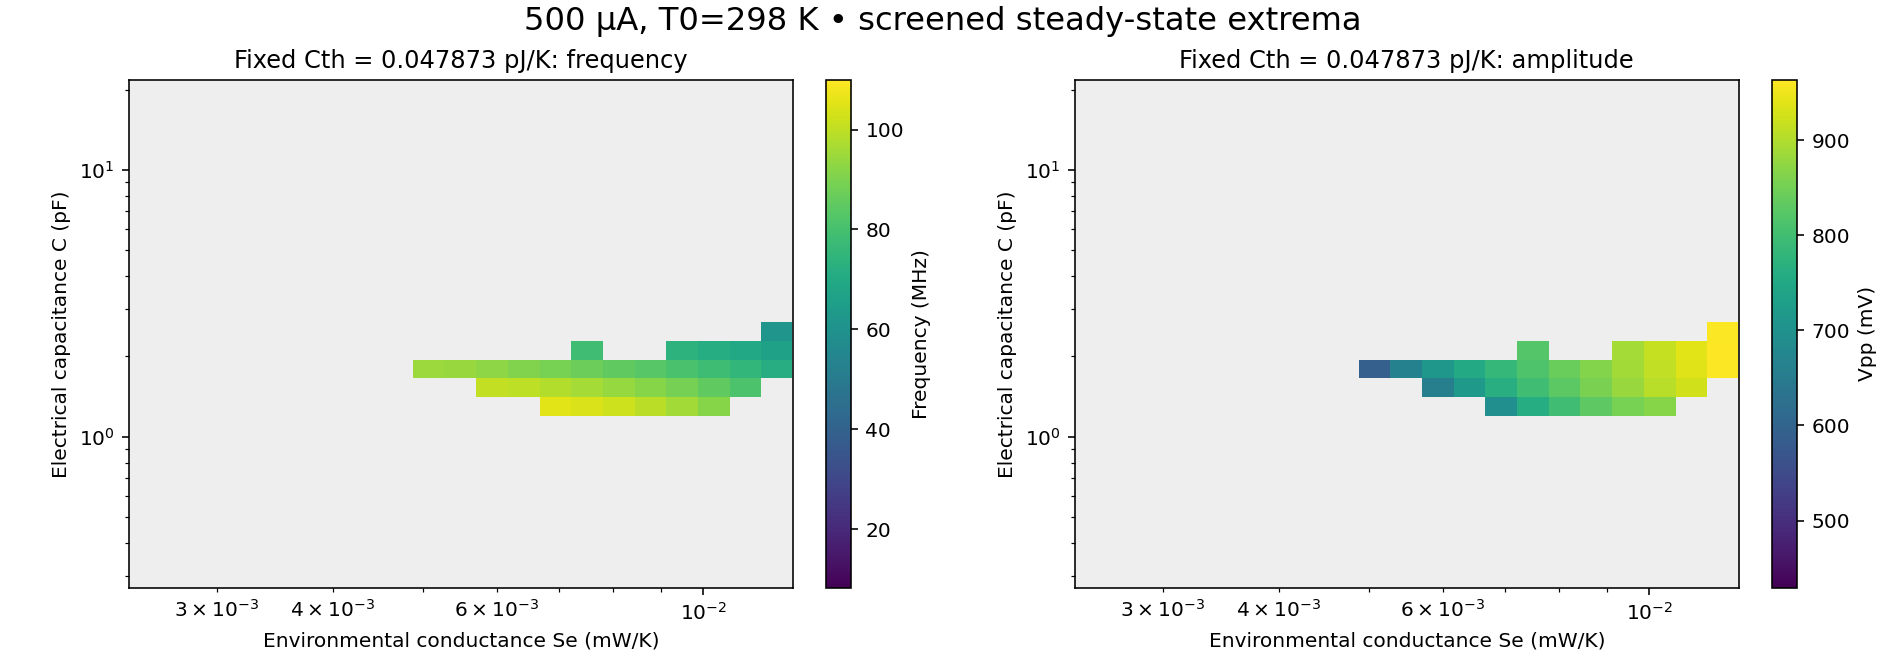
\includegraphics[width=0.88\textwidth,height=0.39\textheight,keepaspectratio]{parameter_exploration_example.png}
\par\footnotesize Example slice: vary \(C\) and \(S_e\) at fixed \(C_{th}\).
\par\vspace{0.10cm}\raggedright\footnotesize
Heatmaps show frequency and peak-to-peak voltage. Sliders fix one parameter while the other two vary;
click a retained point to see its voltage and R(T) animation.
\par\vspace{0.14cm}\centering
\localhtmlbutton{parameter-map}{Open the three-parameter heatmaps and GIFs}
\slidesource{12,167 combinations; 1,258 original retained points. Fixed 500 \(\mu\)A, 298 K, \(\gamma=0.95627\) and fitted R(T). These differ from the experimental replay conditions. Gray cells are excluded/unresolved, not physical boundaries. Viewer 4325d1; source eaf6ab.}
\end{frame}

\begin{frame}{A Sparse Follow-up: Capacitance and Oscillation Timing}
\small
To isolate the effect, test three reference parameter sets and multiply both
capacitances by \(s=0.5,\,1,\,2\), keeping \(S_e\) and the operating conditions fixed.
\[
(C,C_{th})\longrightarrow(sC,sC_{th})
\quad\Rightarrow\quad
V_s(t)=V(t/s),\quad T_s(t)=T(t/s),
\]
\[
\boxed{f_s=f/s,\qquad V_{pp,s}=V_{pp}.}
\]
\centering
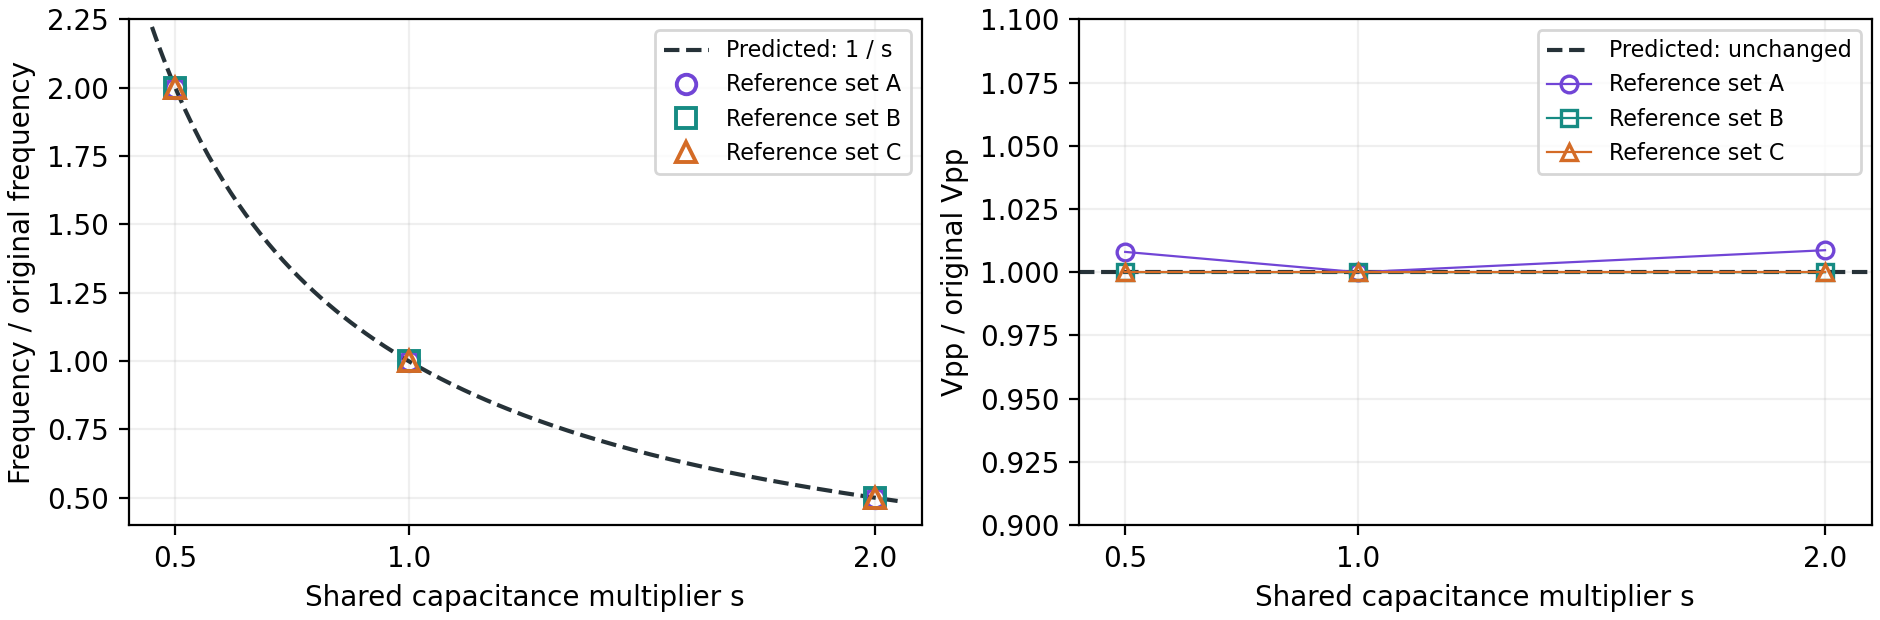
\includegraphics[width=.88\textwidth,height=.38\textheight,keepaspectratio]{controlled_capacitance_scaling.png}
\par\vspace{0.08cm}\raggedright\footnotesize
\textbf{Double both capacitances: half the frequency, with the same voltage--temperature path.}
Changing \(C\) or \(C_{th}\) individually can also change the response shape;
their amplitude effects need not have the same direction.
\slidesource{Constant ideal current 500 \(\mu\)A, 298 K, \(\gamma=0.95627\). Follow-up 3599fb: 12/12 scale checks pass 2\%; plotted points use co-scaled timesteps. Extracted Vpp varies by less than 0.9\% because the feature measurement uses a fixed-time smoothing rule.}
\end{frame}
